\documentclass[sigconf,anonymous,review]{acmart}

\AtBeginDocument{%
  \providecommand\BibTeX{{Bib\TeX}}}

%% Custom preamble (packages, blinding toggle, etc.)
%% Must be before \begin{document} for \usepackage commands.
%% Draft annotations
%% Annotation classes from pandoc/filters/annotations.lua:
%%   .todo | .cite | .formal | .figure | .scaffold | .meta
\usepackage{todonotes}
\usepackage{xcolor}

%% Cut candidates — color tint only, zero geometry change.
%% Active when \if@ACM@review is true (i.e., review class option is set).
%% Toggled off automatically when review option is removed for submission.
\makeatletter
\if@ACM@review
  \newenvironment{cutcandidate}[1][]{%
    \par\begingroup\color{red!50!black}\ignorespaces
  }{\par\endgroup}
\else
  \newenvironment{cutcandidate}[1][]{}{}
\fi
\makeatother

%% Pandoc emits \tightlist for compact lists
\providecommand{\tightlist}{\setlength{\itemsep}{0pt}\setlength{\parskip}{0pt}}

%% Acronyms — auto-generated from pandoc/acronyms.yaml by acronyms.lua
\usepackage{acronym}
%% Auto-generated from pandoc/acronyms.yaml — do not edit.
\acrodef{ARF}[ARF]{Architecture Reference Framework}
\acrodef{BPMN}[BPMN]{Business Process Model and Notation}
\acrodef{CSL}[CSL]{Credential Schema Layer}
\acrodef{DCL}[DCL]{Domain Concept Layer}
\acrodef{DID}[DID]{Decentralized Identifier}
\acrodef{DSE}[DSE]{Design Space Exploration}
\acrodef{EAA}[EAA]{Electronic Attestation of Attributes}
\acrodef{FSL}[FSL]{Format-Specific Layer}
\acrodef{GDPR}[GDPR]{General Data Protection Regulation}
\acrodef{MDE}[MDE]{Model-Driven Engineering}
\acrodef{OCL}[OCL]{Object Constraint Language}
\acrodef{PGM}[PGM]{Partial Graph Modeling}
\acrodef{PID}[PID]{Person Identification Data}
\acrodef{QEAA}[QEAA]{Qualified Electronic Attestation of Attributes}
\acrodef{RDF}[RDF]{Resource Description Framework}
\acrodef{SSI}[SSI]{Self-Sovereign Identity}
\acrodef{VC}[VC]{Verifiable Credential}
\acrodef{VCDM}[VCDM]{Verifiable Credentials Data Model}
\acrodef{ZKP}[ZKP]{zero-knowledge proof}


\usepackage{listings}         % approved
\usepackage{array}            % column formatting (raggedright, arraybackslash)
\usepackage{tabularx}         % auto-width tables for two-column layout
\newcolumntype{L}{>{\raggedright\arraybackslash}X}
%% booktabs is loaded by acmart.cls — no need to load it here

%% Allow line breaks at underscores in \texttt (monospace) text.
%% Without this, long predicate names like supports_multi_credential_proof
%% overflow tabularx columns because LaTeX cannot hyphenate them.
\renewcommand\_{\textunderscore\allowbreak}

% \definecolor{basicColor}{RGB}{105, 108, 119}
\definecolor{basicColor}{RGB}{58, 59, 64}
\definecolor{keywordcolor}{RGB}{27,105,116}
\definecolor{emphColor}{RGB}{166, 38, 164}
\definecolor{commentcolor}{RGB}{160, 161, 167}
\definecolor{stringcolor}{RGB}{80, 161, 79}
\definecolor{segmentColor}{RGB}{0, 86, 84}
\definecolor{switchColor}{RGB}{94, 0, 45}
\definecolor{trackElementColor}{RGB}{107, 107, 107}
\definecolor{relationColor}{RGB}{25, 32, 43}

\newcommand{\kw}[1]{\textsf{\upshape\color{keywordcolor}#1}}
\newcommand{\dslStyle}[1]{\textsf{\upshape\color{emphColor}#1}}
\newcommand{\true}[0]{\kw{1}}
\newcommand{\false}[0]{\kw{0}}


\lstdefinelanguage{refinery}{
	% Refinery language keywords: declarations, predicates, 4-valued logic,
	% control, and builtin types.
	morekeywords={class,abstract,extends,contains,refers,opposite,container,
		enum,pred,error,shadow,propagation,rule,pattern,
		must,may,true,false,unknown,count,exists,equals,default,
		scope,node,import,int,real,string,boolean},
	% Keyword class 2: metamodel type names of this paper, rendered in
	% relationColor. Extend when listings introduce new types.
	morekeywords=[2]{Entity,Prop,Subject,Value,Claim,Credential,CredEntity,
		CredentialSubject,Formatted_Credential,EidasMandate,PrivacyRequirement},
	alsoletter={_},
	otherkeywords={*},
	emph={},
	emphstyle={\color{emphColor}},
	sensitive=true, morecomment=[l]{//}, morecomment=[s]{/*}{*/}, morecomment=[l]{\%},
	morestring=[b]{"}
}
\lstdefinestyle{refinery}{
	basicstyle=\footnotesize\ttfamily\upshape\linespread{0.9}\selectfont,
	aboveskip=4pt,
	belowskip=4pt,
	commentstyle=\color{commentcolor}\ttfamily,
	stringstyle=\color{stringcolor}\ttfamily,
	%frameround=tttt,
	captionpos=b,
	keywordstyle=\color{keywordcolor}\bfseries\ttfamily,
	keywordstyle=[2]\color{relationColor}\bfseries\ttfamily,
	showstringspaces=false,
	tabsize=2,
	language=refinery,
	escapeinside={(*@}{@*)},
	breaklines=true,
	literate=%
	{==>}{$\Longrightarrow$}3
	{<->}{$\longleftrightarrow$}3
	{=:=}{{$=\mathrel{\mkern-9mu}=$}}2
	{<=}{$\leqslant$}1
	{>=}{$\geqslant$}1
	{!=}{{$\mathrel{\ooalign{$\mkern3mu\not$\cr$=\mathrel{\mkern-9mu}=$}}$}}2
}
\newcommand*{\SavedLstInline}{}
\let\SavedLstInline\lstinline
\DeclareRobustCommand*{\lstinline}{%
  \ifmmode
    \let\SavedBGroup\bgroup
    \def\bgroup{%
      \let\bgroup\SavedBGroup
      \hbox\bgroup
    }%
  \fi
  \SavedLstInline
}
\newcommand{\refi}[1]{\textup{\lstinline[style=refinery]{#1}}}

% \begin{lstlisting}[style=refinery]
% //Entry states must not have incoming 
% //transitions.
% error incomingToEntry(Entry e) <->
%     Transition(t),
%     target(t, e).
% \end{lstlisting}

% \refi{error pred foo(a,b)}


%% Rights management information.
\setcopyright{acmlicensed}
\copyrightyear{2026}
% \acmYear{2026}
% \acmDOI{XXXXXXX.XXXXXXX}

\acmConference[MODELS 2026]{ACM/IEEE 29th International Conference on
  Model Driven Engineering Languages and Systems}{October 04--09,
  2026}{Malaga, Spain}
\acmISBN{978-1-4503-XXXX-X/2026/10}

%%\acmSubmissionID{123-A56-BU3}

%%
%% end of the preamble, start of the body of the document source.
\begin{document}

\title[Detecting Cross-Layer Design Errors in VC Ecosystems]{Detecting Cross-Layer Design Errors in Digital Credential Ecosystems with a Layered Metamodel}

%% The "author" command and its associated commands are used to define
%% the authors and their affiliations.
%% Of note is the shared affiliation of the first two authors, and the
%% "authornote" and "authornotemark" commands
%% used to denote shared contribution to the research.
\author{Martin Farkas}
% \authornote{Both authors contributed equally to this research.}
\email{martin.farkas@edu.bme.hu}
\orcid{0000-0003-4260-717X}
\affiliation{%
  \institution{Budapest University of Technology and Economics}
  \city{Budapest}
  \country{Hungary}
}

\author{Kristóf Marussy}
% \authornotemark[1]
\email{marussy@mit.bme.hu}
\orcid{0000-0002-9135-8256}
\affiliation{%
  \institution{Budapest University of Technology and Economics}
  \city{Budapest}
  \country{Hungary}
}

\author{Oszkár Semeráth}
\email{semerath@mit.bme.hu}
\orcid{0000-0002-3592-5105}
\affiliation{%
  \institution{Budapest University of Technology and Economics}
  \city{Budapest}
  \country{Hungary}
}

\author{Zoltán Micskei}
\email{micskeiz@mit.bme.hu}
\orcid{0000-0003-1846-261X}
\affiliation{%
  \institution{Budapest University of Technology and Economics}
  \city{Budapest}
  \country{Hungary}
}

\author{Imre Kocsis}
\email{ikocsis@mit.bme.hu}
\orcid{0000-0002-2792-3572}
\affiliation{%
  \institution{Budapest University of Technology and Economics}
  \city{Budapest}
  \country{Hungary}
}




%%
%% By default, the full list of authors will be used in the page
%% headers. Often, this list is too long, and will overlap
%% other information printed in the page headers. This command allows
%% the author to define a more concise list
%% of authors' names for this purpose.
\renewcommand{\shortauthors}{Farkas et al.}

\begin{abstract}
Emerging digital credential ecosystems allow persons and organizations
to selectively present cryptographically verifiable claims. Such
ecosystems are being deployed under diverse governance frameworks, from
EU Digital Identity Wallets to community-governed decentralized identity
systems, whose design constraints span domain-level claim semantics,
credential schema structure, and format-specific privacy capabilities.
Constraints from W3C standards, EU regulations, and community
specifications interact across layers: their combined effect is not
predictable from any individual source, yet no formal framework checks
their joint consistency.

We present a three-layer metamodel and formalized constraint set for
credential ecosystem design, grounded in the W3C Verifiable Credentials
Data Model 2.0, with cross-layer constraints formalized as graph
predicates in the Refinery partial graph modeling framework. We validate
coverage against the W3C specification, expressiveness against EU
regulatory sources, and error detection against known anti-patterns. The
evaluation shows that constraints from different governance frameworks
can be formally conflicting, and that design errors spanning multiple
layers become visible only through the integrated formalization:
classifying eight eIDAS constraints, formalizing five anti-patterns, and
surfacing two cross-layer errors that no single-layer analysis detects.\end{abstract}


%%
%% CCS codes — generate at https://dl.acm.org/ccs
\begin{CCSXML}
<ccs2012>
   <concept>
       <concept_id>10011007.10011006.10011050</concept_id>
       <concept_desc>Software and its engineering~Context specific languages</concept_desc>
       <concept_significance>300</concept_significance>
       </concept>
   <concept>
       <concept_id>10002978.10002986.10002990</concept_id>
       <concept_desc>Security and privacy~Logic and verification</concept_desc>
       <concept_significance>500</concept_significance>
       </concept>
   <concept>
       <concept_id>10002978.10002986.10002988</concept_id>
       <concept_desc>Security and privacy~Security requirements</concept_desc>
       <concept_significance>500</concept_significance>
       </concept>
   <concept>
       <concept_id>10002978.10002991.10002994</concept_id>
       <concept_desc>Security and privacy~Pseudonymity, anonymity and untraceability</concept_desc>
       <concept_significance>100</concept_significance>
       </concept>
   <concept>
       <concept_id>10011007.10010940.10010971.10010980.10010984</concept_id>
       <concept_desc>Software and its engineering~Model-driven software engineering</concept_desc>
       <concept_significance>500</concept_significance>
       </concept>
   <concept>
       <concept_id>10011007.10010940.10010992.10010998.10003791</concept_id>
       <concept_desc>Software and its engineering~Model checking</concept_desc>
       <concept_significance>300</concept_significance>
       </concept>
 </ccs2012>
\end{CCSXML}

\ccsdesc[300]{Software and its engineering~Context specific languages}
\ccsdesc[500]{Security and privacy~Logic and verification}
\ccsdesc[500]{Security and privacy~Security requirements}
\ccsdesc[100]{Security and privacy~Pseudonymity, anonymity and untraceability}
\ccsdesc[500]{Software and its engineering~Model-driven software engineering}
\ccsdesc[300]{Software and its engineering~Model checking}

\keywords{metamodeling, verifiable credentials, design space exploration,
  partial models, graph constraints}

%% Teaser figure moved to Section 3 (Overview)

%\received{27 March 2026} % Suppressed for anonymous review submission

\maketitle

%% === Content sections (generated from sections/*.md by build.sh) ===
\section{Introduction}\label{sec:introduction}

When a civil registry, a land registry, and an employer each issue digital credentials that can be used for a government housing subsidy, covering family status, property records, and income respectively, the bank processing the application must accept all three in a single eligibility check. EU regulation mandates a specific credential format for government attestations \citep{eidas2}. Data protection law requires that privacy-sensitive checks disclose only the minimum necessary information \citep{gdpr}; an income threshold check should not require revealing the exact value, yet the mandated format lacks this capability while other standardized formats provide it. No existing modeling tool is available to detect this and similar requirement conflicts. These credentials are tamper-evident, cryptographically verifiable claims exchanged between issuers, holders, and verifiers as defined by the W3C Verifiable Credentials Data Model 2.0 \citep{sporny_verifiable_2025}; designing their ecosystems requires satisfying constraints that span what claims mean, how credentials are structured, and what each format can express.

Credential ecosystem designs can contain errors undetectable by single-layer inspection because governance frameworks impose requirements that conflict across abstraction layers \citep{mazzocca_survey_2025}. The W3C Verifiable Credentials Data Model defines structural conformance rules that standard credentials must satisfy \citep{sporny_verifiable_2025}. The eIDAS Architecture and Reference Framework mandates specific credential formats for government-issued attestations \citep{noauthor_eu-digital-identity-walleteudi-doc-architecture-and-reference-framework_2026}. The General Data Protection Regulation requires data minimization \citep{gdpr}, operationalized in this paper as a format capability requirement: a threshold comparison should not require disclosing the underlying value. Unlike hierarchical requirement systems where constraints decompose top-down, credential governance sources are non-cooperating peers with competing goals; their requirements cannot necessarily be brought into a coherent whole.

Existing tools operate at a single layer: JSON Schema validators check credential structure, format-specific conformance tools verify encoding constraints, governance frameworks define requirements in isolation. None checks cross-layer consistency. In the housing subsidy scenario, the income credential's format assignment, structural conformance, and privacy requirement each pass their respective single-layer checks, yet their combination is unsatisfiable. A credential schema may be well-formed when inspected in isolation, yet violate a cross-layer constraint that links domain-level claim semantics to format-specific privacy capabilities. Detecting such errors requires a formalization that spans all three concern spaces.

We make the following contributions:

\begin{enumerate}
\def\labelenumi{\arabic{enumi}.}
\tightlist
\item
  A \textbf{three-layer metamodel} for credential ecosystem design, grounded in the W3C Verifiable Credentials Data Model 2.0, spanning claim properties, credential schemas, and format-specific representations.
\item
  A \textbf{formalization of cross-layer constraints} as predicates in the Refinery partial graph modeling framework.
\item
  A \textbf{three-axis validation} demonstrating metamodel coverage against the W3C specification, constraint expressiveness against W3C and EU regulatory sources, and error detection against known credential design anti-patterns. The validation detects two cross-layer design errors, a governance conflict and a format expressiveness gap, undetectable by single-layer analysis.
\end{enumerate}

Cross-layer constraints are formalized as graph predicates in Refinery \citep{marussy_refinery_2024}. Refinery's solver reveals when constraints from different governance frameworks are formally contradictory and generates valid alternative designs when they are not. The framework supports three usage modes: \emph{consistency checking} confirms that a design satisfies all constraints, \emph{error identification} names specific violations, and \emph{design space exploration} generates valid configurations or proves that none exist. \autoref{fig:teaser} illustrates the complete pipeline on a housing subsidy credential scenario that serves as the running example throughout.

\autoref{sec:background} introduces the W3C \ac{VCDM} 2.0, multi-layer modeling, and the Refinery graph modeling tool, which provides the formal apparatus for the cross-layer analysis. \autoref{sec:overview} develops a housing subsidy scenario in which credentials from three independent authorities fall under conflicting governance mandates, and defines the three usage modalities that set the requirements the formalization must satisfy. \autoref{sec:approach} formalizes the three-layer metamodel and its cross-layer constraints as Refinery graph predicates grounded in the running example. \autoref{sec:evaluation} validates the metamodel against the W3C specification, EU regulatory sources, and solver scalability. \autoref{sec:related-work} positions the contribution against credential ecosystem formalization and model-driven security engineering, and \autoref{sec:conclusion} examines the design-time scope boundary and identifies extensions to runtime verification.

\section{Background}\label{background}

\label{sec:background}

\subsection{W3C Verifiable Credentials Data Model 2.0}\label{w3c-verifiable-credentials-data-model-2.0}

\label{sec:vcdm}

The W3C \acf{VCDM} 2.0 \citep{sporny_verifiable_2025} defines a verifiable credential as a tamper-evident set of claims made by an issuer about one or more credential subjects. A \emph{claim} is a subject--property--value triple asserting a characteristic of the credential subject, for example that an applicant's monthly income exceeds a threshold. The \emph{issuer} is the entity asserting the claims; the \emph{holder} possesses the credential and presents it to a \emph{verifier}. Each credential carries a digital signature or comparable cryptographic evidence that binds the claims to the issuer and allows a verifier to confirm their integrity. VCDM 2.0 standardizes this structural vocabulary: the abstract data model for credential issuance, holding, and verification. It does not, however, prescribe the domain-level semantics of claim values, the encoding format in which credentials are serialized, or the privacy capabilities available during presentation. This gap between structural vocabulary and the domain-specific, format-specific concerns that govern real deployments motivates the multi-layer separation developed in \autoref{sec:approach}.

VCDM credentials can be secured and serialized in multiple formats with distinct cryptographic foundations and privacy capabilities. SD-JWT-VC \citep{terbu_sd-jwt-based_2026} provides hash-based \emph{selective disclosure}, allowing a holder to reveal a chosen subset of claims while withholding others. AnonCreds \citep{curran2022anoncreds} uses Camenisch--Lysyanskaya signatures to support both selective disclosure and \emph{predicate proofs}, \acp{ZKP} that a claim value satisfies a given predicate (e.g., \refi{monthly_income} \(\geq\) \refi{threshold}) without disclosing the value itself. JSON-LD credentials with Data Integrity Proofs \citep{noauthor_verifiable_2024} support selective disclosure via the BBS cryptosuite \citep{_bbs_2024} but currently lack predicate proof capability (the underlying BBS+ scheme admits extensions that could support them). The ISO 18013-5 mobile document format (mdoc) \citep{_mobile_2021} is mandated alongside SD-JWT-VC by the eIDAS 2.0 \ac{ARF} for EU wallet attestations \citep{noauthor_eu-digital-identity-walleteudi-doc-architecture-and-reference-framework_2026}; since both formats lack predicate proof support, subsequent sections use SD-JWT-VC as the representative format.

\subsection{Multi-Layer Modeling}\label{multi-layer-modeling}

\label{sec:multi-layer}

Multi-layer modeling organizes a design problem into abstraction layers, each defining its own types, instances, and well-formedness rules. Multi-level metamodeling \citep{goos_essence_2001} relates such layers through successive instantiation controlled by potency annotations. The three layers in \autoref{sec:approach} (domain concepts, credential schemas, and format-specific representations) are abstraction layers in this sense, but they are not related by instantiation. Each layer is an independently governed concern space whose constraints originate from distinct normative sources not designed for joint satisfaction. Cross-layer relationships are formalized as typed trace references and graph predicates over partial models (\autoref{sec:cross-layer}), not as potency annotations.

Layer definitions in \autoref{sec:approach} use Ecore-style class diagrams with typed references and containment hierarchies as the metamodeling notation. Layer instance(s) are \emph{partial models}: model elements may have definite (\refi{must}), absent (\refi{must not}), or open (\refi{unknown}) status for any reference or class membership, enabling reasoning over specifications where not all design decisions have been made. Cross-layer trace relationships are formalized as typed references between partial models at adjacent layers, capturing the correspondence between a domain concept and the credential-layer claims that represent it.

\subsection{Partial Graph Modeling with Refinery}\label{partial-graph-modeling-with-refinery}

\label{sec:refinery}

\todo[inline]{Do not use this PGM, it is a non-existing concept}

\acf{PGM}
During the early phase of developement, our knowledge about models is often incomplete. In partial modeling

\todo[inline]{cite this: Partial models: Towards modeling and reasoning with uncertainty \\
M Famelis, R Salay, M Chechik}

uncertainty can be denoted explicitly, thus a range of design alternatives can be developed together.
Refinery \citep{marussy_refinery_2024} is a modeling methodology in which design specifications are expressed as partial models and graph predicates serve as a first-class constraint language. Refinery uses a four-valued logic interpretation

\todo[inline]{cite this: \\
@incollection{Belnap77useful, \\
author = {Belnap, Jr., Nuel D.}, \\
title = {A Useful Four-Valued Logic}, \\
booktitle = {Modern Uses of Multiple-Valued Logic}, \\
series = {EPIS}, \\
volume = {2}, \\
pages = {5-37}, \\
year = {1977}, \\
publisher = {Springer}, \\
doi = {10.1007/978-94-010-1161-7\_2} \\
}}

to every node, edge, attribute value, enabling reasoning over incomplete (or inconsistent) specifications where both structural and data-level decisions remain open. In Refinery, nodes correspond to objects (instances of classes defined in a metamodel), and edges correspond to typed references between objects; class membership is an additional unary relation over nodes.

\todo[inline,color=green!20]{formal: Oscar: precise definition of graph elements (nodes, edges, class membership as relations). Reference Marussy et al. 2024. Target length: 2--3 sentences.}

A \emph{4-valued partial model} provide partial interpretation to edge and class memberships in a model.

\todo[inline]{Honnan jn ez a commited?}

The four-valued interpretation assigns each element one of four statuses: \refi{true} (the value must be true), \refi{false} (the value must be false), \refi{unknown} (possibly true or false), and \refi{error} (both true and false, denoting contraiction). In diagrams,

\todo[inline]{do we have diagrams?}

a solid line denotes true values, a dashed line denotes unknown values, and absence denotes a false value. During the development (or automated synthesis) of partial models, \refi{unknown} values are gradually refined to either \refi{true} or \refi{false}. If a model contains only \refi{true} and \refi{false} values, we call them \emph{concrete models}. If one of the design decision contradicts a design constraint, it produces \refi{error} to show the contradiction between a decision and the regulation.

\todo[inline,color=green!20]{formal: Oscar: refinement ordering definition (partial model A refines B iff every must/must-not commitment in B is preserved in A). Target length: 1--2 sentences + definition.}

\autoref{lst:refinery-metamodel} illustrates a fragment of the domain concept layer from \autoref{sec:approach}, simplified for exposition.\footnote{The full metamodel in \autoref{sec:approach} uses a symmetric \refi{neighbours} relation and the error predicate \refi{non_connected}; the simplified names here prioritize readability.} Classes define node types with typed references; the \refi{contains} keyword denotes ownership (composition). The derived predicate \refi{reachable} pattern-matches over the \refi{property} and \refi{value} references: it holds when entity \(a\) owns a property whose value is entity \(b\). The \emph{error predicate} \refi{disconnected} uses transitive closure (\refi{+}) to flag any pair of entities not connected by a chain of reachable steps; when it evaluates to \refi{must}, the partial model contains a structural flaw that no refinement can repair.

Graph predicates define structural constraints and derived properties over partial models. A predicate body specifies a graph pattern; the framework evaluates it over the partial interpretation under the four-valued semantics introduced above. Negation and transitive closure extend this evaluation to richer structural queries.

\todo[inline,color=green!20]{formal: Oscar: predicate evaluation semantics over partial interpretations. How four-valued logic lifts to predicate bodies, negation, transitive closure. Target length: 3--5 sentences or a compact table.}

\begin{lstlisting}[style=refinery, caption={Metamodel fragment with error predicate}, label=lst:refinery-metamodel]
abstract class Entity {
    contains Prop[] property
}
class Subject extends Entity.
class Value extends Entity.

class Prop {
    contains Value[1] value
}

pred reachable(Entity a, Entity b) <->
    property(a, p), value(p, b).

error disconnected(Entity a, Entity b) <->
    a != b, !reachable+(a, b).
\end{lstlisting}

\emph{Propagation rules} derive new facts during refinement: when their precondition pattern matches with all elements committed (\refi{must}), the consequent is applied. A propagation rule with a positive consequent (e.g., \refi{Subject(e)}) infers new class memberships or edges. \emph{Negative elimination} is the dual: a propagation rule with a negated consequent (e.g., \refi{!value(p, e)}) removes design choices that would necessarily violate a constraint, setting them to \refi{must not}. Both operate incrementally during model refinement, narrowing the space of possible completions before generation explores them.

\todo[inline,color=green!20]{formal: Oscar: propagation rule semantics (precondition = must pattern, consequent = forced assignment). Boolean encoding and fixpoint computation. Target length: 3--5 sentences.}

\autoref{lst:refinery-mechanisms} demonstrates the remaining mechanisms. The propagation rule \refi{classify_root} performs positive inference: when an entity has no incoming \refi{value} reference, it is classified as a \refi{Subject}. The rule \refi{no_self_loop} performs negative elimination: when an entity owns a property, that property cannot point back to the same entity as its value. The \emph{shadow predicate} \refi{DCL} marks all entities and properties as belonging to the domain concept layer; it records derived information for inspection without constraining generation. Finally, the \emph{scope constraint} bounds the number of instances of each type, controlling the size and shape of generated models.

\begin{lstlisting}[style=refinery, caption={Propagation rules, shadow predicate, and scope constraint}, label=lst:refinery-mechanisms]
propagation rule classify_root(Entity e) <->
    must !value(_, e)
==>
    Subject(e).

propagation rule no_self_loop(Prop p, Entity e) <->
    must property(e, p)
==>
    !value(p, e).

shadow pred DCL(e) <-> Entity(e); Prop(e).

scope Entity = 3..5, Prop = 2..4.
\end{lstlisting}

Given a partial specification combining a metamodel, predicates, and instance-level assertions, Refinery applies propagation rules to derive new facts, checks error predicates, and generates concrete models that satisfy all constraints, or determines that no consistent completion exists \citep{semerath_graph_2018}. Generation is refinement-based: every generated model is guaranteed to satisfy all specified constraints (soundness), and if a constraint is violated in every possible completion, the tool detects the violation (completeness).

\todo[inline,color=green!20]{formal: Oscar: formal statement of soundness and completeness guarantees for Refinery's refinement-based generation. Reference Semerath et al. 2018. Target length: 2--3 sentences + formal claim.}

In credential ecosystem design, requirements arrive incrementally from independent governance sources from evolving stand and regulatory frameworks are adopted, so the designer must reason over partial specifications. \ac{PGM} evaluates constraints \emph{during} refinement of such partial specifications, pruning inconsistent design choices before they propagate (\autoref{sec:rw-multilevel} compares this to bounded model finding alternatives).

\todo[inline,color=gray!10]{meta: Section: Background / Sec 2.3 \\
Budget: was ~0.35 pages, now ~0.75--0.85 pages before Oscar's additions. Total Sec 2  1.45 pages (0.2 over 1.25 budget). Oscar's formal content will add further; page cuts needed elsewhere.}

\section{Overview}\label{sec:overview}

The housing subsidy scenario in \autoref{sec:motivation} exhibits both types of cross-layer design error the formalization detects: a vertical governance conflict on a single credential's format assignment, and a horizontal capability gap spanning two credentials (\autoref{sec:headlines}). \autoref{sec:functional-overview} defines the three usage modes the framework must support.

\subsection{Motivation}\label{sec:motivation}

Consider a government housing subsidy where eligibility requires credentials from three independent authorities: family status from a civil registry, property records from a land registry, and income from an employer.\footnote{Based on the Hungarian Family Housing Subsidy (Családi Otthonteremtési Kedvezmény, CSOK), simplified. Additional credentials required in practice (tax clearance, criminal record check) are omitted; these involve simple status checks that do not introduce cross-credential arithmetic or predicate proof requirements, and their inclusion would not affect the headline results.} The required property size depends on the number of children \citep{noauthor_5182023_2023} (the decree prescribes minimum floor areas of 40, 50, 60, 70, and 80 m² for one through five or more children, respectively), a constraint that spans two credentials, and the income check must satisfy both EU format mandates and data protection requirements.

\autoref{fig:teaser} illustrates this scenario across three metamodel layers. At the domain concept layer, the applicant's facts (number of children, property floor area, monthly income) form an information graph with domain-level constraints: the minimum floor area is a function of the number of children \citep{noauthor_5182023_2023}, and income must exceed a regulatory threshold. At the credential schema layer, these facts are distributed across three credentials issued by independent authorities, each with its own credential subject. All three subjects must be aligned (they refer to the same applicant) and each claim must trace to the corresponding domain-level property. At the format-specific layer, EU regulations mandate specific credential formats for government-issued attestations \citep{noauthor_eu-digital-identity-walleteudi-doc-architecture-and-reference-framework_2026}, while data protection law's minimization principle, operationalized here as a credential-layer requirement, implies that privacy-sensitive checks such as whether income exceeds a threshold should not require disclosing the underlying value \citep{gdpr}.\footnote{A directly analogous enforcement action supports this operationalization: the Hungarian data protection authority (NAIH) fined a bank 35M HUF for copying applicants' entire pregnancy booklets when only a 12-week gestation threshold check was required for a subsidized loan, finding the collection grossly disproportionate \citep{noauthor_naih_2020}.}

Inspected in isolation, each layer is well-formed: domain properties, credential schemas, and format assignments each pass their own validation. Cross-layer analysis, however, reveals two problems. The income credential cannot simultaneously satisfy the eIDAS \ac{ARF} format mandate (requiring SD-JWT-VC \citep{noauthor_eu-digital-identity-walleteudi-doc-architecture-and-reference-framework_2026}) and \ac{GDPR} data minimization (requiring predicate proof capability \citep{gdpr}); SD-JWT-VC supports selective disclosure but not predicate proofs. The floor area constraint requires cross-credential predicate evaluation spanning two credentials, which no widely used format supports in zero-knowledge. Neither problem is visible when any single layer is inspected alone.

The constraints in this scenario originate from governance frameworks that were not designed to be jointly satisfied: W3C VCDM \citep{sporny_verifiable_2025} defines structural conformance rules for credentials, the eIDAS \ac{ARF} \citep{noauthor_eu-digital-identity-walleteudi-doc-architecture-and-reference-framework_2026} mandates specific credential formats for government attestations, \ac{GDPR} \citep{gdpr} requires data minimization, and format specifications \citep{terbu_sd-jwt-based_2026, curran2022anoncreds} define what each format can and cannot express. These sources were enacted independently; no single source anticipates the constraints imposed by the others.

The remainder of this section defines a framework that captures constraints across these layers and governance sources and demonstrates how it can be used by a designer.

\begin{figure*}[t]
  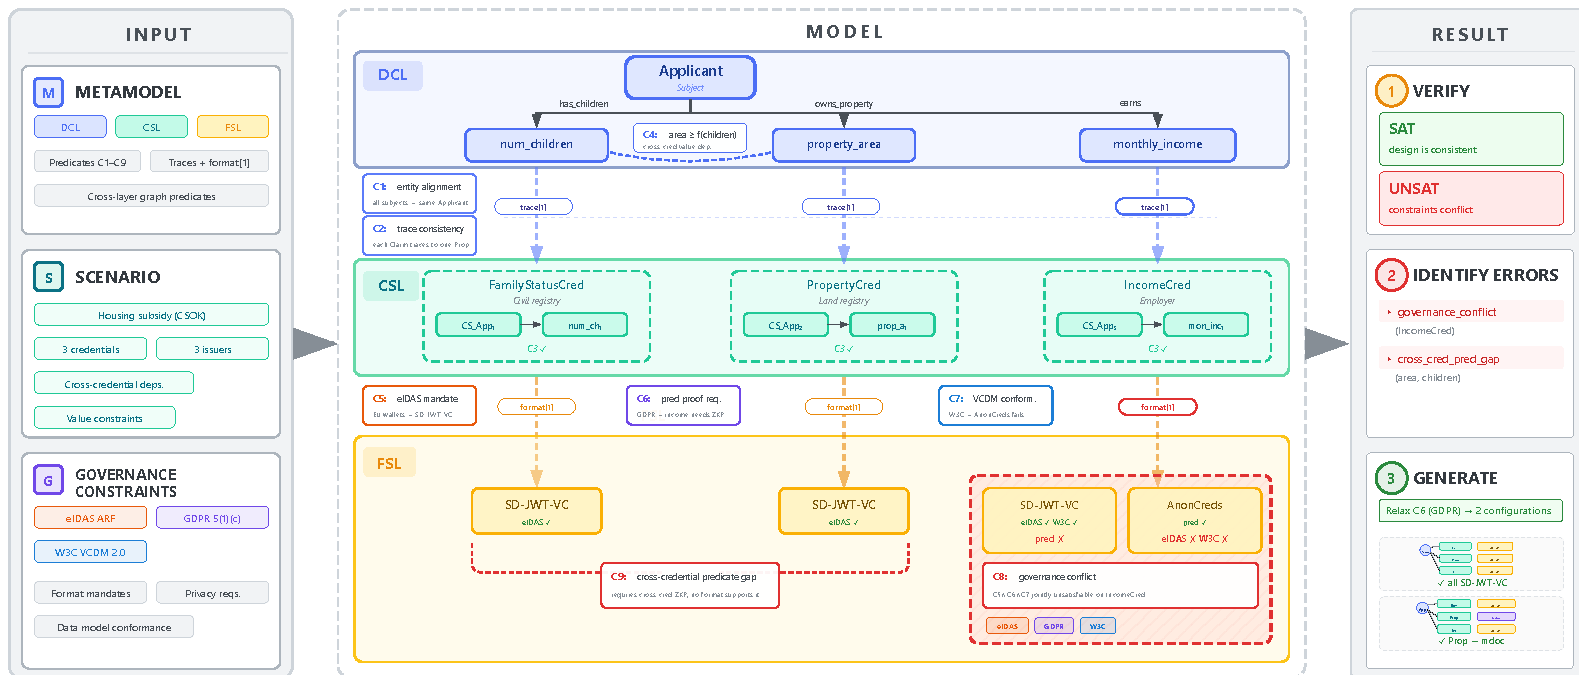
\includegraphics[width=\textwidth]{assets/teaser.pdf}
  \caption{The proposed multi-layer modeling framework applied to a housing subsidy credential ecosystem across three metamodel layers, from domain facts through credential schemas to format-specific representations. Error identification detects conflicting governance requirements on the income credential; design space exploration confirms no valid format assignment exists. Both results require cross-layer analysis.}
  \Description{Teaser figure description.}
  \label{fig:teaser}
\end{figure*}

\subsection{Functional Overview}\label{sec:functional-overview}

\autoref{fig:teaser} illustrates the framework on the housing subsidy scenario. A credential ecosystem designer provides a \emph{partial design}: the ecosystem's entities, credentials, and their relationships, together with governance constraints from regulatory and technical sources. Some choices, such as format assignments, may be left open for the framework to resolve. The metamodel (\autoref{sec:approach}) organizes design elements across three layers, and cross-layer constraints, expressed as graph predicates, are evaluated by the Refinery partial graph modeling framework \citep{marussy_refinery_2024}.

The framework supports three usage modes. \emph{Consistency checking} confirms that a complete design satisfies all constraints. \emph{Error identification} pinpoints which constraints conflict and where; in the housing subsidy scenario, it reports that the income credential's format assignment simultaneously violates a governance mandate and a data protection requirement (\autoref{fig:teaser}). When the designer leaves choices open, \acf{DSE} generates diverse valid completions\footnote{Refinery's diversity mechanism yields meaningfully distinct graph completions; the designer inspects a representative sample rather than an exhaustive enumeration.} or proves that no satisfying configuration exists. A typical workflow chains these modes: the designer runs error identification to discover the income credential conflict, restructures the income claim as a pre-computed boolean, then runs \ac{DSE} to search for valid format assignments.

\section{Approach}\label{sec:approach}

Credential ecosystem design involves three distinct concerns: what domain-level facts exist and how they relate, how those facts are grouped into credentials with defined subjects and claims, and which concrete credential format each credential uses. The metamodel separates these concerns into three layers: the \acf{DCL}, the \acf{CSL}, and the \acf{FSL}. The layered structure follows the multi-layer modeling principles introduced in \autoref{sec:multi-layer}: each layer is derived from the one above and carries its own intra-layer constraints. Constraints within and across layers are formalized as graph predicates that the Refinery framework (\autoref{sec:refinery}) can evaluate, yielding the three usage modes defined in \autoref{sec:functional-overview}. \autoref{fig:metamodel} shows the complete metamodel; the definitions below correspond to its elements layer by layer. Full Refinery encodings for all layer definitions, propagation rules, and constraint predicates are provided in the supplementary material.

\subsection{Domain Concept Layer}\label{sec:dcl}

Domain-level facts are modeled as a typed information graph at the first layer. The abstract metaclass \refi{Entity} has two concrete subclasses: \refi{Subject} and \refi{Value}. A \refi{Subject} is an entity that can anchor a credential, representing the person, organization, or thing about which claims are made. A \refi{Value} is an entity that serves as the target of a property. Each \refi{Entity} contains zero or more \refi{Prop} instances; each \refi{Prop} holds exactly one \refi{Value} through a containment reference and carries a trace link to the credential schema layer (\autoref{sec:csl}). The ternary predicate \refi{statement(s, p, v)} is satisfied when subject \(s\) owns property \(p\) and \(p\) contains value \(v\), with the well-formedness condition \(s \neq v\). The distinction between \refi{Subject} and \refi{Value} is inferred structurally: a propagation rule (\autoref{sec:refinery}) classifies any \refi{Entity} with no incoming value reference as a \refi{Subject}: a root of the property tree, and therefore a candidate credential subject at the \ac{CSL} layer.
A credential ecosystem must cover all domain-level facts; an entity unreachable from the rest of the graph represents a fact that no credential path connects to the subject, and therefore cannot be verified. The \refi{non_connected} error predicate (\autoref{sec:refinery}) enforces this: it flags any pair of entities not transitively reachable through the \refi{neighbours} relation, where two entities are neighbours if a \refi{statement} connects them in either direction. The \refi{no_self_loop} propagation rule prevents an entity from serving as both the owner and the value of the same property, a structurally meaningless configuration that would collapse the subject--value distinction. Together with the \(s \neq v\) condition in the \refi{statement} predicate, these constraints ensure that every \ac{DCL} instance is a connected, directed acyclic information graph with clear directionality from subjects to values. The \refi{cyclic} error predicate enforces acyclicity via transitive closure of the \refi{neighbours} relation. In terms of the usage modes (\autoref{sec:functional-overview}), \ac{DCL} constraints serve error identification: evaluating \refi{non_connected} on a partial specification with an orphaned entity returns \textbf{NOT\_OK}(\refi{non_connected(e1, e2)}), naming the unreachable pair and indicating where the domain model is incomplete.

In the housing subsidy scenario (\autoref{fig:teaser}, top), the \ac{DCL} instance models the Applicant as a \refi{Subject} with three properties: \refi{has_children} \(\to\) \refi{num_children} (family size), \refi{owns_property} \(\to\) \refi{property_area} (floor area), and \refi{earns} \(\to\) \refi{monthly_income} (employment income). Three statements capture the domain facts, one per property edge in the domain graph. Two domain constraints apply: \refi{property_area} \(\geq\) \refi{min_area(num_children)} links two properties across what will become separate credentials, and \refi{monthly_income} \(\geq\) \refi{threshold} establishes a privacy-sensitive eligibility check. All claim-layer structural constraints (connectivity, no self-loops) are satisfied.

\subsection{Credential Schema Layer}\label{sec:csl}

The \acf{CSL} models the partitioning of domain-level facts into credentials, each issued by a different authority and carrying a subset of the domain's claims. Each \ac{CSL} element is traced from a \ac{DCL} element: the abstract metaclass \refi{CredEntity} carries a mandatory \refi{trace} reference to exactly one \ac{DCL} \refi{Entity}, and each \ac{DCL} \refi{Prop} contains exactly one \refi{Claim} via \refi{Prop::trace}. This pair of cross-layer references ensures that every credential-layer element has a domain-level origin (\autoref{fig:metamodel}). \ac{CSL} mirrors the \ac{DCL} type structure: \refi{CredentialSubject} and \refi{CredentialValue} specialize \refi{CredEntity}, paralleling \ac{DCL}'s \refi{Subject} and \refi{Value}. A \refi{Claim} connects a source \refi{CredEntity} to a target \refi{CredentialValue}, mirroring the \ac{DCL} \refi{statement} predicate. Each \refi{CredentialSubject} optionally contains a \refi{Credential}, which itself holds exactly one \refi{Formatted_Credential} (\autoref{sec:fsl}).

Trace mappings do more than record provenance. Combined with Refinery's propagation rules, they actively derive \ac{CSL} structure from \ac{DCL} during model generation. Two propagation rules derive \ac{CSL} type assignments from \ac{DCL} structure. \refi{subject_traces_to_subject} infers \refi{CredentialSubject} when a \refi{CredEntity} traces to a \ac{DCL} \refi{Subject}; \refi{root_is_cred_subj} infers it when no \refi{Claim} targets the entity, mirroring the \ac{DCL} \refi{root_is_subj} at the credential level. The effect is that \ac{CSL} type assignments are derived from \ac{DCL} structure rather than independently specified: a credential entity's type is a consequence of its domain-layer origin.

Beyond type derivation, the metamodel enforces structural well-formedness through four predicates (two shadow, two error; \autoref{sec:refinery}). The shadow predicates mirror \ac{DCL} structure at the credential level: \refi{credential_statement} is true when a \refi{Claim} connects distinct source and target with the target typed as \refi{CredentialValue}; \refi{Root_cred_entity} holds when a \refi{CredEntity} is not targeted by any \refi{credential_statement}. The error predicates flag structural violations: \refi{no_empty_cred} flags a \refi{CredentialSubject} with no outgoing \refi{Claim}, and \refi{root_ent_doesnt_have_cred} flags a root entity without an associated \refi{Credential}; the anti-pattern catalog (\autoref{sec:anti-patterns}) classifies all five predicates by layer scope and kind. The error predicates catch structural violations that would otherwise propagate silently to downstream format assignment. When either fires, the framework reports the violation (e.g., \textbf{NOT\_OK}(\refi{no_empty_cred(cs)})) before format-specific constraints are even evaluated. In terms of the usage modes (\autoref{sec:functional-overview}), the shadow predicates (\refi{credential_statement}, \refi{Root_cred_entity}) derive structural facts in all three modes; the error predicates (\refi{no_empty_cred}, \refi{root_ent_doesnt_have_cred}) trigger in consistency checking and error identification.

In the housing subsidy scenario, three credentials partition the facts: FamilyStatusCred (civil registry: \refi{CS_Applicant}\(_1\), claim \refi{has_children}\(_1 \to\) \refi{num_children}\(_1\)), PropertyCred (land registry: \refi{CS_Applicant}\(_2\), claim \refi{owns_property}\(_1 \to\) \refi{property_area}\(_1\)), and IncomeCred (employer: \refi{CS_Applicant}\(_3\), claim \refi{earns}\(_1 \to\) \refi{monthly_income}\(_1\)). Each credential subject, claim, and value traces to its \ac{DCL} counterpart.

All three credential subjects trace to the same \ac{DCL} entity: \refi{trace(CS_Applicant_i, Applicant)} for \(i \in \{1,2,3\}\). Each claim traces to its corresponding property, and each credential value traces to its corresponding value. Entity alignment holds pairwise: \refi{aligned(CS_Applicant_i, CS_Applicant_j)} for all \(i \neq j\). The cross-property domain constraint (minimum floor area as a function of the number of children) now spans two credentials, requiring the verifier to combine claims from FamilyStatusCred and PropertyCred.

\subsection{Format-Specific Layer}\label{sec:fsl}

Each credential receives a concrete representation format at the third layer, the \acf{FSL}. The abstract metaclass \refi{Formatted_Credential} has five concrete subclasses (one per credential format in scope: AnonCreds, JSON-LD, JWT-VC, SD-JWT-VC, and mdoc), and each \refi{Credential} contains exactly one instance via the \refi{format[1]} containment. These formats differ along a design-relevant axis: \emph{selective disclosure} (revealing a subset of claims) versus \emph{predicate proofs} (proving a comparison such as \refi{monthly_income} \(\geq\) \refi{threshold} without disclosing the value). Format capabilities follow from the analysis in \autoref{sec:vcdm}: only AnonCreds supports predicate proofs natively; the remaining formats provide selective disclosure only. Formats lacking predicate proofs force issuers to pre-compute boolean claims, restructuring the domain concept layer (\autoref{sec:cross-layer}). Unlike the \ac{DCL} and \ac{CSL}, the format-specific layer does not yet carry intra-layer structural constraints; its role in the metamodel is different. \ac{FSL} elements participate in cross-layer predicates (\autoref{sec:cross-layer}), carry governance annotations as typed containment, and their capability predicates feed the propagation rules that narrow the format design space during generation. The layer is a metamodel component with cross-layer predicate participation and governance semantics, not a lookup table mapping credentials to format labels.

The metamodel encodes format capabilities as six derived predicates over the class hierarchy, each capturing a functional property that at least one governance framework or domain requirement in the running example imposes:

\begin{table}[htb]
\caption{\ac{FSL} capability predicates derived from the format class hierarchy.}
\small
\setlength{\tabcolsep}{4pt}
\begin{tabularx}{\columnwidth}{LL}
\toprule
Predicate & Capability \\
\midrule
{supports\_predicate\_proof} & Predicate proof (e.g., {monthly\_income} \(\geq\) {threshold} without
disclosure) \\
{supports\_selective\_disclosure} & Selective disclosure of claim subsets \\
{conforms\_vcdm} & W3C VCDM 2.0 data model conformance \\
{supports\_zkp} & Zero-knowledge proof support \\
{supports\_offline\_verification} & Offline verification without network access \\
{supports\_multi\_credential\_proof} & Cross-credential predicate evaluation \\
\bottomrule
\end{tabularx}
\end{table}

Propagation rules narrow the format design space during generation: requiring predicate proof support on IncomeCred eliminates all formats except AnonCreds, which does not conform to W3C \ac{VCDM} 2.0, setting up the governance conflict in \autoref{sec:headlines}. Three governance annotation classes (\refi{EidasMandate}, \refi{PrivacyRequirement}, \refi{VcdmConformance}) attach regulatory requirements to individual credentials as typed markers for error identification and \ac{DSE}.

In the housing subsidy scenario, format assignments are governance-driven. FamilyStatusCred and PropertyCred are assigned SD-JWT-VC under the eIDAS \ac{ARF} mandate; both formats mandated by the \ac{ARF} (SD-JWT-VC and mdoc) lack predicate proof support; we use SD-JWT-VC as representative \citep{noauthor_eu-digital-identity-walleteudi-doc-architecture-and-reference-framework_2026}. IncomeCred is the conflict site analyzed in \autoref{sec:headlines}: the income threshold check requires predicate proof capability that the ARF-mandated format does not provide.

\subsection{Cross-Layer Constraints as Graph Predicates}\label{sec:cross-layer}

\begin{figure}
\centering

\includegraphics[width=1\linewidth,height=\textheight,keepaspectratio,alt={The three-layer type graph. The  models facts as a typed information graph; the  partitions facts into credentials with subject bindings and trace mappings; the  assigns concrete formats with capability predicates and governance annotations.}]{pandoc/assets/fig_metamodel.pdf}
\caption{The three-layer type graph. The \ac{DCL} models facts as a typed information graph; the \ac{CSL} partitions facts into credentials with subject bindings and trace mappings; the \ac{FSL} assigns concrete formats with capability predicates and governance annotations.}\label{fig:metamodel}
\end{figure}

Cross-layer constraints are predicates whose variables reference elements from more than one metamodel layer; they capture design requirements that no single-layer check can express. The following table classifies the constraints exercised in the housing subsidy scenario by source and scope:

\begin{table}[htb]
\caption{Cross-layer constraint taxonomy. C1--C3 are metamodel-enforced; C4 is
grounded in regulation; C5--C7 originate from independent governance
frameworks; C8 and C9 are cross-layer results.
\label{tab:constraint_taxonomy}}
\small
\setlength{\tabcolsep}{4pt}
\begin{tabularx}{\columnwidth}{LLLL}
\toprule
\# & Constraint & Source & Layers \\
\midrule
C1 & Entity alignment & Structural & DCL\(\leftrightarrow\)CSL \\
C2 & Trace consistency & Structural & DCL\(\rightarrow\)CSL \\
C3 & No empty credential & Structural & CSL \\
C4 & Cross-credential value dep. & Domain rule & DCL horiz. \\
C5 & Format mandate & eIDAS \ac{ARF} & FSL \\
C6 & Predicate proof required & \ac{GDPR} Art. 5(1)(c) & DCL\(\leftrightarrow\)FSL \\
C7 & VCDM conformance & W3C VCDM 2.0 & CSL\(\leftrightarrow\)FSL \\
C8 & \textbf{Governance conflict} & eIDAS+GDPR+W3C & FSL \\
C9 & Cross-credential predicate gap & Format limitation & DCL\(\leftrightarrow\)FSL \\
\bottomrule
\end{tabularx}
\end{table}

Constraints C1--C3 are structural (metamodel-enforced). C4 is a domain rule grounded in government regulation. C5--C7 each originate from a different governance framework. C8 and C9 are cross-layer results: they emerge only when constraints from multiple sources and layers are checked jointly. \autoref{sec:headlines} develops C8 and C9 as the paper's headline results.

\autoref{fig:teaser} traces all three usage modes on the constraint table above. Consistency checking on the partial specification returns \textbf{OK}. Fixing IncomeCred to SD-JWT-VC triggers error identification: the framework returns \textbf{NOT\_OK}(\refi{governance_conflict(IncomeCred, income_format)}), naming the conflict site where C5, C6, and C7 cannot be simultaneously satisfied. Leaving IncomeCred's format open and running \ac{DSE} with \refi{C5} \(\wedge\) \refi{C6} \(\wedge\) \refi{C7} returns \textbf{UNVIABLE}. Relaxing C6, the framework generates configurations assigning SD-JWT-VC to all three credentials.

The predicates defined in the preceding sections (\refi{non_connected}, \refi{no_empty_cred}, \refi{root_ent_doesnt_have_cred}) operate within a single layer using the Refinery mechanisms introduced in \autoref{sec:refinery}. The cross-layer predicates below combine elements from multiple layers and fall into three categories defined in \autoref{sec:refinery}: \emph{propagation rules}, \emph{shadow predicates}, and \emph{error predicates}. This classification determines which usage mode (\autoref{sec:functional-overview}) each predicate serves.

A \refi{Claim} that connects to a \refi{CredEntity} tracing to the wrong \ac{DCL} \refi{Entity} is a silent design error: each layer is well-formed individually, but the cross-layer mapping is broken. Two propagation rules prevent this by negative elimination. The target consistency rule enforces that if \refi{trace(p, c)} and \refi{value(p, e)} hold (where \refi{trace(p, c)} denotes \refi{Prop::trace} and \refi{trace(t, e)} below denotes \refi{CredEntity::trace}), then any \refi{CredEntity} \(t\) for which \(\neg\)\refi{trace(t, e)} holds is excluded as \(c\)'s target; the source rule is dual over \refi{property(e, p)}. In the running example, the \refi{Claim} tracing to \refi{has_children} can only target a \refi{CredEntity} tracing to \refi{num_children}, not one tracing to \refi{property_area}. Both rules operate by negative elimination (\autoref{sec:refinery}): bindings inconsistent with committed traces are excluded before generation explores them.

The shadow predicate \refi{aligned} formalizes cross-authority subject identity: \refi{aligned(ce1, ce2)} holds when two distinct \refi{CredEntity} instances satisfy \refi{trace(ce1, e)} \(\wedge\) \refi{trace(ce2, e)} for some \ac{DCL} \refi{Entity} \(e\). In the running example, \refi{aligned(CS_Applicant_i, CS_Applicant_j)} holds for all \(i \neq j\). A second shadow predicate, \refi{common_parent}, holds when two \refi{Prop} instances' traced \refi{Claim} instances share a source \refi{CredEntity}, capturing co-location within a single credential. Both feed the anti-pattern analysis (\autoref{sec:evaluation}); \refi{aligned} additionally feeds \refi{cross_cred_predicate_gap} below.

Some design problems are invisible at any single layer. When a domain constraint spans two credentials (\refi{property_area} \(\geq\) \refi{f(num_children)} requires combining claims from FamilyStatusCred and PropertyCred), the design depends on a format capability that may not exist. The shadow predicate \refi{cross_cred_predicate_gap} detects this: \refi{cross_cred_predicate_gap(c1, c2)} fires when \refi{aligned(cs1, cs2)} and at least one credential's format lacks multi-credential proof support. No deployed format supports cross-credential arithmetic (AnonCreds supports multi-credential \emph{presentation} but not cross-credential \emph{computation}), so the predicate fires for every aligned pair, making a structural limitation of the current format space visible. As a shadow predicate, it records a condition whose severity depends on domain requirements; \autoref{sec:headlines} develops this as the second headline result.

Format capability propagation rules apply the same negative elimination mechanism (\autoref{sec:refinery}) at the format level. When a governance annotation demands a capability, incompatible format classes are eliminated: requiring \refi{supports_predicate_proof} on IncomeCred excludes SD-JWT-VC, JWT-VC, mdoc, and JSON-LD, leaving only AnonCreds. When no format in scope satisfies a required capability, the only workaround is restructuring the domain concept layer, replacing a numeric property with pre-computed boolean claims, a cross-layer design consequence that \autoref{sec:headlines} develops as the first headline result.

\section{Evaluation}\label{evaluation}

\label{sec:evaluation}

We evaluate the metamodel and its cross-layer constraint formalization along two complementary axes. A qualitative \emph{elaboration} (\autoref{sec:elaboration}) characterizes metamodel coverage against the W3C VCDM 2.0 specification, constraint expressiveness against EU regulatory sources, two headline results --- a governance conflict and a format expressiveness gap --- demonstrating cross-layer constraint value, a catalog of structural anti-patterns, and a baseline comparison against single-layer alternatives. A quantitative \emph{scalability measurement} (\autoref{sec:scalability}) benchmarks three Refinery solver operations across ecosystem sizes up to 30 credentials.

\subsection{Elaboration}\label{elaboration}

\label{sec:elaboration}

\subsubsection{Metamodel Coverage}\label{metamodel-coverage}

\label{sec:coverage}

We characterize the metamodel's coverage of W3C VCDM 2.0 concepts \citep{sporny_verifiable_2025} as a soundness--completeness pair. For soundness, every metaclass and capability predicate traces to a VCDM concept: DCL metaclasses formalize the claim-level information structure, CSL metaclasses the credential packaging model, and FSL format classes with six capability predicates the format properties relevant to governance constraint evaluation. For completeness, the metamodel deliberately excludes three VCDM concept families outside credential \emph{schema design}: proof mechanisms (cryptographic, orthogonal to structural modeling), verifiable presentations (runtime protocols), and credential status (lifecycle management). These are scope boundaries of the design-time formalization, not limitations of the graph predicate approach. These three families govern how a credential with a given structure is used (signed, presented, revoked), not how that structure is designed. Governance constraints from independent sources (eIDAS, GDPR, W3C) bear on structure and format assignment; formalizing these at design time is what makes cross-source conflicts detectable.

\subsubsection{Constraint Expressiveness}\label{constraint-expressiveness}

\label{sec:expressiveness}

We collected eight normative constraints from the eIDAS Architecture Reference Framework (ARF) v2.7.3 \citep{noauthor_eu-digital-identity-walleteudi-doc-architecture-and-reference-framework_2026} governing credential format assignment, and classified each as \emph{fully expressible}, \emph{partially expressible}, or \emph{not expressible}. Three are fully expressible (\autoref{tab:expressiveness}), five partially, and none falls entirely outside the metamodel's capacity. The full constraint analysis is provided in the supplementary material.

\begin{table}
\caption{Fully expressible eIDAS ARF constraints. Each maps directly to metamodel
predicates or architecture. \label{tab:expressiveness}}
\small
\setlength{\tabcolsep}{4pt}
\begin{tabularx}{\columnwidth}{LLLL}
\toprule
ID & Constraint & Source & Predicate / Mechanism \\
\midrule
ARF-C1 & PID must be issued in both ISO 18013-5 and SD-JWT-VC & PID\_02 & \texttt{EidasMandate} annotation + format class membership \\
ARF-C4 & Proximity presentation requires mdoc format & ARB\_02 & \texttt{supports\_offline\_verification}; propagation rule eliminates
SD-JWT-VC \\
ARF-C7 & Attributes defined encoding-independently, then per-format & ARB\_06 & DCL\(\to\)CSL\(\to\)FSL layer architecture \\
\bottomrule
\end{tabularx}
\end{table}

The five partially expressible constraints share two root causes. Three constraints (ARF-C2, C3: qualified vs.~non-qualified attestation format restrictions; ARF-C6: VCDM completeness as a meta-level property) condition format eligibility on the credential qualification level (PID, QEAA, or non-qualified EAA in eIDAS terminology), but the metamodel does not yet distinguish these attestation subtypes. Two constraints (ARF-C5: per-claim selective disclosability; ARF-C8: salted-hash vs.~ZKP-based selective disclosure) require privacy annotations at claim granularity rather than format level. Both gaps are closable by extending the metaclass hierarchy; neither requires changing the constraint formalization approach. A constraint falls outside the metamodel's capacity only when it governs runtime behavior (revocation timing, holder-binding protocols) with no design-time structural counterpart --- none of the eight falls into this category.

\emph{Remark.} ARF-C7 provides external validation of the metamodel's layered architecture. The ARF requires that attestation attributes be defined encoding-independently before being specified per-format (ARB\_06 \citep{noauthor_eu-digital-identity-walleteudi-doc-architecture-and-reference-framework_2026}). The metamodel was designed from the W3C VCDM structure, not from the ARF; that the EU governance framework independently mandates the same DCL\(\to\)CSL\(\to\)FSL separation confirms the layering reflects a structural property of credential ecosystem design rather than an artifact of the formalization.

\subsubsection{Headline Results}\label{headline-results}

\label{sec:headlines}

\paragraph{Headline 1: Income governance conflict (vertical)}\label{headline-1-income-governance-conflict-vertical}

At the credential schema layer, IncomeCred is well-formed: \(\text{CS\_Applicant}_3\) traces to Applicant, \(\text{earns}_1\) traces to the \(\text{earns}\) property, \(\text{monthly\_income}_1\) traces to its value. All structural constraints (C1--C3) are satisfied.

At the format-specific layer, three governance sources impose requirements on IncomeCred:

\begin{enumerate}
\def\labelenumi{\arabic{enumi}.}
\tightlist
\item
  \textbf{eIDAS ARF} (normative, SHALL): \(\text{format}(\text{IncomeCred}) \in \{\text{SD-JWT-VC}, \text{mdoc}\}\) --- neither supports predicate proofs \citep{noauthor_eu-digital-identity-walleteudi-doc-architecture-and-reference-framework_2026}.
\item
  \textbf{GDPR Art. 5(1)(c)} (authors' operationalization): the income threshold check requires disclosing only whether \(\text{monthly\_income} \geq \text{threshold}\), not the exact value. We interpret the data minimization principle as requiring that, when a threshold comparison suffices, disclosing the exact value constitutes disproportionate data collection --- and that enforcing this at the credential layer requires predicate proof capability \citep{gdpr}. Neither inferential step is self-evident: the first is a reading of data minimization for threshold-check scenarios; the second assumes minimization must be achieved through technical means at the credential layer rather than through organizational or procedural controls. A directly analogous enforcement action illustrates the operational weight of this principle: the Hungarian data protection authority (NAIH) fined a bank 35M HUF for copying applicants' entire pregnancy booklets when only a 12-week gestation threshold check was required for a subsidized loan. NAIH found the collection grossly disproportionate \citep{noauthor_naih_2020}, establishing that collecting exact values when a threshold check suffices violates data minimization --- precisely the scenario that predicate proofs address at the credential layer.
\item
  \textbf{W3C VCDM 2.0}: the credential format must conform to the VCDM data model --- AnonCreds v1 does not, as its encoding is designed around the CL signature scheme rather than VCDM's data model \citep{sporny_verifiable_2025} \citep{curran2022anoncreds}.
\end{enumerate}

No format satisfies all three requirements. SD-JWT-VC satisfies (1) and (3) but not (2). AnonCreds satisfies (2) but not (1) or (3). The configuration is unsatisfiable: constraints C5, C6, and C7 cannot be simultaneously satisfied on IncomeCred.

This contradiction is invisible to single-layer inspection. At the credential schema layer alone, IncomeCred is well-formed. At the format-specific layer under the eIDAS ARF alone, SD-JWT-VC is compliant. At the format-specific layer under GDPR alone, AnonCreds provides the needed capability. Only the joint, cross-governance, cross-layer analysis reveals the conflict.

\emph{Remark.} An issuer-precomputed boolean claim (\(\text{income\_above\_threshold}: \text{true}\)) can approximate a predicate proof within SD-JWT-VC. However, this workaround requires the issuer to anticipate every verifier threshold at issuance time, produces combinatorial explosion for multi-threshold scenarios, and remains static --- a credential issued with threshold \(X\) cannot serve a verifier requiring threshold \(Y\) without reissuance. As shown in \autoref{sec:cross-layer}, this workaround restructures the domain concept layer --- itself a cross-layer propagation that confirms the need for multi-layer analysis.

\paragraph{Headline 2: Cross-credential predicate gap (horizontal)}\label{headline-2-cross-credential-predicate-gap-horizontal}

The domain constraint \(\text{property\_area} \geq \text{min\_area}(\text{num\_children})\) (C4) requires combining values from two credentials issued by independent authorities: \(\text{property\_area}\) from PropertyCred (land registry) and \(\text{num\_children}\) from FamilyStatusCred (civil registry).

No credential format with a stable specification and production-ready implementations supports cross-credential arithmetic predicates in zero-knowledge. Among the five such formats (SD-JWT-VC, JSON-LD with BBS+, JWT-VC, mdoc, AnonCreds v1), only AnonCreds v1 offers any predicate support --- single-credential range proofs (\(\text{attr} \geq \text{const}\)) under CL signatures --- but even it cannot combine values across credentials issued by independent authorities. ZK-SNARK-based research prototypes such as zk-creds \citep{rosenberg_zk-creds_2023} demonstrate cross-credential predicates but lack EU wallet ecosystem adoption and W3C VCDM conformance. AnonCreds v2 plans BBS+ signature support with range proof capabilities, but no stable specification is available for independent verification.

To verify the floor area constraint, the verifier must see both raw values from two separate credentials, defeating the privacy properties that ZKP-capable formats promise. The metamodel captures this: a domain-concept-layer constraint (C4) that spans credentials cannot be enforced privacy-preservingly at the format-specific layer because no deployed format supports cross-credential predicate proofs (C9).

This gap is again invisible to single-layer inspection: the domain concept layer constraint is well-defined, both credentials are well-formed at the credential schema layer, and each credential's format is individually valid at the format-specific layer. Only the cross-layer analysis --- checking whether the DCL constraint can be enforced given the FSL format capabilities --- reveals the expressiveness gap.

\emph{Complementarity.} The two results are orthogonal. Headline 1 identifies a \emph{vertical} governance conflict: contradictory requirements on a single credential's format from different regulatory sources. Headline 2 identifies a \emph{horizontal} expressiveness gap: an ecosystem-level constraint spanning credentials that exceeds any single format's capabilities. Together, they demonstrate that multi-layer analysis detects both governance conflicts and format expressiveness gaps invisible to single-layer inspection.

\subsubsection{Anti-Pattern Detection}\label{anti-pattern-detection}

\label{sec:anti-patterns}

\autoref{tab:antipatterns} catalogues five structural anti-patterns formalized as graph predicates over the partial model.

\begin{center}
\small
\setlength{\tabcolsep}{4pt}
\begin{tabularx}{\columnwidth}{LLLLL}
\toprule
Anti-pattern & Description & Graph predicate & Layer(s) & Kind \\
\midrule
Disconnected domain graph & Entity pair not transitively reachable & \texttt{non\_connected} & DCL & error \\
Empty credential & \texttt{CredentialSubject} with no outgoing \texttt{Claim} & \texttt{no\_empty\_cred} & CSL & error \\
Orphaned root entity & Root \texttt{CredEntity} without associated \texttt{Credential} & \texttt{root\_ent\_doesnt\_have\_cred} & CSL & error \\
Trace misalignment & \texttt{Claim} target traces to wrong DCL \texttt{Entity} & \texttt{prop\_t} / \texttt{prop\_s} & DCL\(\leftrightarrow\)CSL & propagation \\
Cross-credential predicate gap & Aligned credential pair lacks cross-credential proof support & \texttt{cross\_cred\_predicate\_gap} & DCL\(\leftrightarrow\)FSL & shadow \\
\bottomrule
\end{tabularx}
\end{center}

\label{tab:antipatterns}

The first three anti-patterns are detectable by single-layer inspection: \texttt{non\_connected} operates within the DCL, \texttt{no\_empty\_cred} and \texttt{root\_ent\_doesnt\_have\_cred} within the CSL. Trace misalignment requires cross-layer analysis. Each layer is individually well-formed, but the propagation rules \texttt{prop\_t} and \texttt{prop\_s} eliminate any binding where a \texttt{Claim}`s target \texttt{CredEntity} traces to a different DCL \texttt{Entity} than the \texttt{Prop} it was derived from. The cross-credential predicate gap is invisible at any single layer: the domain constraint is well-defined at the DCL, both credentials are structurally valid at the CSL, and each format is individually compliant at the FSL. Only the cross-layer shadow predicate, which checks \texttt{aligned} credential subjects against their formats' \texttt{supports\_multi\_credential\_proof} capability, surfaces the gap. This graduated visibility, from intra-layer errors through cross-layer trace inconsistencies to ecosystem-level capability gaps, is the central argument for multi-layer formalization over single-layer alternatives. The catalog is extensible: adding an anti-pattern requires a new graph predicate over the existing metamodel, not structural changes to layers or trace links.

\subsubsection{Baseline Comparison}\label{baseline-comparison}

\label{sec:baseline}

The multi-layer advantage for cross-layer detection is partly definitional. The comparison's purpose is to identify which issue classes fall into this detection gap and to confirm that current practice cannot cover them. We compare analytically against three baselines of increasing formality; no existing tool implements cross-layer credential ecosystem checking, so the comparison is structural rather than empirical. Manual expert review, the current industry practice for credential ecosystem design, can identify single-credential format conflicts but lacks systematic coverage of cross-credential dependencies and provides no guarantee that all governance sources have been jointly checked. Formalization adds systematicity: the model checks all constraint combinations exhaustively (the G0--G7 sensitivity experiment confirms only the full conjunction produces unsatisfiability), scales beyond what manual analysis can track, and yields a reproducible artifact. Single-layer metamodeling (e.g., a UML class diagram with OCL constraints per layer) detects intra-layer structural violations such as empty credentials or disconnected domain graphs, but cannot express the cross-layer trace predicates (\texttt{prop\_t}, \texttt{prop\_s}) or the cross-layer capability checks (\texttt{cross\_cred\_predicate\_gap}) that link domain constraints to format capabilities. Only the integrated multi-layer formalization with cross-layer graph predicates detects all five anti-pattern categories, including the two headline results (\autoref{sec:headlines}) that are invisible to any single-layer approach. No alternative multi-layer credential ecosystem formalization exists in the literature; the three baselines represent the state of practice, not a weakened comparison set.

\subsection{Scalability Measurement}\label{scalability-measurement}

\label{sec:scalability}

We evaluate the scalability of the Refinery-based formalization across three solver operations of increasing cost. \emph{Consistency checking} (\texttt{check} in Refinery) verifies that the partial model specification has no internal contradictions. \emph{Concretizability checking} (\texttt{check\ -k}) goes further: it determines whether a concrete model satisfying all constraints, including error predicates, exists --- this is the operation that detects governance conflicts such as the income format unsatisfiability in \autoref{sec:headlines}. \emph{Model generation} (\texttt{generate}) produces a fully resolved model instance, enumerating valid credential ecosystem designs for design space exploration. We measure all three to answer two research questions. \textbf{RQ1:} How does conflict detection (concretizability checking) scale with model size? \textbf{RQ2:} How does design space exploration (model generation) scale with model size? Consistency checking serves as a baseline: it should scale well but cannot detect cross-layer conflicts, because the partial model is internally consistent even when no valid concretization exists.

We construct synthetic instances from \(N{=}1\) to \(N{=}30\) credentials. Each credential contributes one \texttt{Prop}--\texttt{Value} pair at the DCL, one \texttt{CredentialSubject}--\texttt{Claim}--\texttt{CredentialValue}--\texttt{Credential} group at the CSL, and one \texttt{Formatted\_Credential} node at the FSL, yielding a total of 11 to 272 graph nodes (\autoref{tab:scalability}). All credential subjects trace to a shared \texttt{Subject}; the last credential's format class is left unresolved for the solver. Each scale point has two variants: a satisfiable (SAT) variant without governance conflicts, and an unsatisfiable (UNSAT) variant that imports the Headline 1 governance conflict predicate, requiring the solver to detect that no format assignment satisfies all three governance frameworks simultaneously. As a secondary \emph{constraint sensitivity} experiment, we fix \(N{=}3\) and vary governance framework combinations over the power-set \(\mathcal{P}(\{\text{eIDAS}, \text{Privacy}, \text{VCDM}\})\), yielding eight configurations (G0--G7). Instance definitions and Refinery encodings are provided as supplementary material.

All instances are evaluated using the Refinery CLI,\footnote{Container image \texttt{ghcr.io/graphs4value/refinery-cli}, pulled via Docker.} where each invocation starts a fresh JVM inside a Docker container. We use Hyperfine as the benchmarking harness with 10 measured runs and 1 warmup run per configuration, on an AMD Ryzen 9 7950X3D (16 cores), 96 GB RAM, Windows 11. Cold JVM startup inside the Docker container adds a constant overhead of \({\approx}3.9\text{s}\) per invocation (measured via a no-op baseline instance); reported times subtract this overhead to isolate solver computation. At small scales (\(N \leq 5\)), solver time is below the measurement noise floor (\({\approx}0.1\text{s}\)). The measurement script, generated instances, and the metamodel source are provided as supplementary material for independent reproduction.

\begin{figure*}
\centering
\fbox{\parbox{0.85\textwidth}{\centering\vspace{2cm}\small Scalability plot: wall-clock time (s) vs.\ model size ($N$ credentials). Lines: consistency check, concretizability-SAT, concretizability-UNSAT, model generation-SAT.\vspace{2cm}}}
\caption{Runtime of three Refinery solver operations across ecosystem sizes from $N{=}1$ to $N{=}30$ credentials. Consistency checking serves as baseline; concretizability checking detects governance conflicts; model generation produces valid configurations.}
\label{fig:scalability}
\end{figure*}

\begin{table}
\caption{Scalability measurements for two Refinery operations, baseline-corrected
(3.9s Docker+JVM overhead subtracted). \emph{Concretizability}
(\texttt{check\ -k}): determines whether a concrete model satisfying all
constraints exists. \emph{Generation} (\texttt{generate}): produces a
concrete model instance. Seconds, mean \(\pm\sigma\) over 10 runs.
\label{tab:scalability}}
\small
\begin{tabular}{rrrrr}
\toprule
\(N\) & \(|V|\) & SAT (s) & UNSAT (s) & Generation (s) \\
\midrule
1 & 11 & \({<}0.1\) & \({<}0.1\) & \(0.55 \pm 0.11\) \\
3 & 29 & \({<}0.1\) & \(0.18 \pm 0.07\) & \(0.56 \pm 0.05\) \\
5 & 47 & \(0.13 \pm 0.10\) & \(0.11 \pm 0.05\) & \(0.69 \pm 0.08\) \\
10 & 92 & \(0.14 \pm 0.05\) & \(0.22 \pm 0.07\) & \(0.77 \pm 0.06\) \\
15 & 137 & \(0.42 \pm 0.12\) & \(0.40 \pm 0.08\) & \(0.94 \pm 0.05\) \\
20 & 182 & \(0.51 \pm 0.06\) & \(0.58 \pm 0.09\) & \(1.23 \pm 0.07\) \\
30 & 272 & \(1.09 \pm 0.06\) & \(1.19 \pm 0.06\) & \(1.85 \pm 0.07\) \\
\bottomrule
\end{tabular}
\end{table}

\textbf{RQ1} (conflict detection scaling): Concretizability checking scales sublinearly with model size, rising from below the measurement noise floor at \(N{=}1\) to 1.09,s at \(N{=}30\) (SAT). SAT and UNSAT instances exhibit comparable timing at each scale point, with differences within measurement noise (\(\sigma\)); at the largest scale (\(N{=}30\)), the UNSAT overhead is 0.10,s, confirming that unsatisfiability detection does not incur significant additional cost. At \(N{=}30\) (272 graph nodes), conflict detection completes in under 1.2,s --- well within interactive use for credential ecosystem sizes an order of magnitude beyond current EU wallet specifications. \textbf{RQ2} (design space exploration scaling): Model generation follows the same growth trend, rising from 0.55,s to 1.85,s. The higher baseline reflects the cost of producing a fully resolved model instance rather than merely determining satisfiability.

\begin{table}
\caption{Constraint sensitivity at \(N{=}3\): governance framework power-set.
Result column reports concretizability (\texttt{check\ -k}). All
configurations complete in under 0.1s of solver time (below the
measurement noise floor at this scale). \label{tab:sensitivity}}
\small
\setlength{\tabcolsep}{4pt}
\begin{tabularx}{\columnwidth}{LcccL}
\toprule
Config & eIDAS & Privacy & VCDM & Result \\
\midrule
G0 &  &  &  & SAT \\
G1 & x &  &  & SAT \\
G2 &  & x &  & SAT \\
G3 &  &  & x & SAT \\
G4 & x & x &  & SAT \\
G5 & x &  & x & SAT \\
G6 &  & x & x & SAT \\
G7 & x & x & x & UNSAT \\
\bottomrule
\end{tabularx}
\end{table}

The constraint sensitivity experiment confirms that only G7, the conjunction of all three governance frameworks, yields unsatisfiability; all seven proper subsets are satisfiable (\autoref{tab:sensitivity}). This validates the Headline 1 finding (\autoref{sec:headlines}): the income governance conflict requires the simultaneous imposition of eIDAS ARF format mandates \citep{noauthor_eu-digital-identity-walleteudi-doc-architecture-and-reference-framework_2026}, GDPR data minimization requirements \citep{gdpr}, and W3C VCDM conformance \citep{sporny_verifiable_2025}. No proper subset of these three sources produces a conflict. The measurements cover \(N\) up to 30 credentials (272 graph nodes); for reference, the EU Digital Identity Wallet Architecture Reference Framework defines fewer than 10 attestation types in its current version \citep{noauthor_eu-digital-identity-walleteudi-doc-architecture-and-reference-framework_2026}, though future ecosystem growth may increase this number. The contribution is the metamodel and its cross-layer constraint formalization; Refinery serves as the validation vehicle, and absolute performance numbers are tool-specific.

\subsection{Threats to Validity}\label{threats-to-validity}

\label{sec:threats}

\paragraph{Construct validity}\label{construct-validity}

The metamodel formalizes credential \emph{schema design}, not the full credential lifecycle. Three VCDM 2.0 concept families fall outside this scope: proof mechanisms (cryptographic layer, orthogonal to structural modeling), verifiable presentations (runtime holder-verifier protocols), and credential status (issuance and revocation lifecycle). These boundaries constrain the class of expressible governance requirements to those that condition format assignment on structural or capability properties of credentials. Within this scope, five of eight eIDAS ARF constraints are classified as partially expressible (\autoref{sec:expressiveness}). The two root causes are a missing attestation-type subclass hierarchy (three constraints condition format eligibility on credential qualification level) and per-claim rather than per-format privacy annotation (two constraints require claim-level selective disclosure control). Both gaps are closable by metaclass extension without changing the constraint formalization approach, but the partially-expressible classification itself rests on our judgment of what constitutes a structural versus a runtime property. Additionally, the DCL's structural inference rule classifies any Entity with no incoming value reference as a Subject; if a modeler omits a property edge by mistake, the entity may be silently promoted to Subject rather than flagged as incomplete.

\paragraph{Internal validity}\label{internal-validity}

The running example (housing subsidy) was selected for structural completeness: it exhibits both a vertical governance conflict (Headline 1) and a horizontal expressiveness gap (Headline 2) within a single, independently documented domain. A randomly sampled credential ecosystem might expose neither or might expose interaction patterns not covered by the current anti-pattern catalog (\autoref{sec:anti-patterns}). The eight eIDAS ARF constraints were extracted from a specific version (ARF v2.7.3 \citep{noauthor_eu-digital-identity-walleteudi-doc-architecture-and-reference-framework_2026}); the constraint landscape may shift as the regulatory framework evolves. Format capability predicates depend on the characterization being both complete and current: an emerging format with novel capability combinations (e.g., BBS+ credentials with partial predicate support) would require extending the format class hierarchy and the derived propagation rules. The scalability instances grow by adding credentials with uniform structure (one property per credential, shared subject), which reflects the common multi-issuer credential ecosystem pattern but does not exercise deeper claim hierarchies or multi-subject credentials that may arise in domains such as healthcare or supply chain management.

\paragraph{External validity}\label{external-validity}

The evaluation operates within a single governance context: EU regulations (eIDAS 2.0 \citep{noauthor_eu-digital-identity-walleteudi-doc-architecture-and-reference-framework_2026}, GDPR \citep{gdpr}) applied to Hungarian administrative procedures. The \texttt{GovernanceAnnotation} mechanism is designed to be governance-agnostic: new regulatory sources require adding annotation subclasses and error predicates, not restructuring the three-layer architecture. However, the evaluation demonstrates this only for the EU context. Governance traditions that impose constraints not reducible to format-capability requirements, such as organizational trust hierarchies or issuer accreditation rules, would require extending the metamodel beyond annotation markers. The single-domain scenario exercises a three-credential, single-subject ecosystem; domains with richer claim structures or multi-subject credentials may stress different metamodel elements. The intended user is a credential ecosystem designer who specifies the domain graph, credential decomposition, and governance requirements in a graph-based formalism; whether a domain expert without metamodeling experience could use the approach effectively remains untested.

\paragraph{Conclusion validity}\label{conclusion-validity}

The scalability instances are synthetic: each adds a credential with one property to the preceding configuration. This linear, homogeneous growth pattern is representative of the common case where independent issuers each contribute one credential to a shared ecosystem, but it does not capture ecosystems where a few credentials carry many claims while others are minimal. Concretizability checking scales sublinearly over the measured range, though growth is uneven --- a step around \(N{=}15\) suggests phase transition behavior in the solver's search strategy. Model generation also scales sublinearly (3.4\(\times\) increase across a 25\(\times\) growth in model size), though superlinear growth may emerge at larger scales as the combinatorial format assignment search dominates. The constraint sensitivity analysis partially compensates for the homogeneous scaling by varying governance complexity at fixed model size, but the power-set covers three governance frameworks only. Refinery-specific performance results establish that the formalization is computationally feasible at practical ecosystem scales; they do not generalize to other partial modeling tools. The contribution is the metamodel and its cross-layer constraints, with Refinery as the validation vehicle. Model definitions, constraint encodings, and all measurement artifacts are provided as supplementary material for independent reproduction.

\todo[inline,color=gray!10]{meta: Dependencies: Sections 04 (what we do), 05 (what we demonstrate).}

\todo[inline,color=gray!10]{meta: Note: Double-blind. CSCS 2024 short paper referenced in third person.}

\todo[inline,color=gray!10]{meta: Source: Gap analysis synthesis (2026-03-25), archive/gap analyis/GAP\_ANALYSIS\_SYNTHESIS.md}

\section{Related Work}\label{related-work}

\label{sec:related-work}

\subsection{Credential Ecosystem Design and Formalization}\label{credential-ecosystem-design-and-formalization}

\label{sec:rw-credential}

Verifiable credential schema design is currently guided by specifications that define credential structure at individual abstraction layers: the W3C Verifiable Credentials Data Model 2.0 \citep{manu_verifiable_2025} and EU Architecture Reference Framework \citep{noauthor_eu-digital-identity-walleteudi-doc-architecture-and-reference-framework_2026} prescribe issuance and presentation flows, while AnonCreds \citep{curran2022anoncreds} and ISO mDL \citep{_mobile_2021} define format-specific encoding and proof mechanisms. \cutcandidate[supplementary survey reference — can be removed for budget]{Mazzocca et al. \citep{mazzocca_survey_2025} provide a comprehensive survey of this landscape.} None of these specifications provides a formal mechanism for checking constraints that span multiple layers. Where formal methods have been applied, they target individual layers: Braun and Käfer \citep{curry_rdf-based_2025} define RDF-based semantics for selective disclosure and zero-knowledge proofs on verifiable credentials, Yamamoto et al. \citep{yamamoto_formalising_2022} formalize selective disclosure specifically for linked-data credentials, and Braun et al. \citep{braun_ssi_2024} verify SSI protocol security properties using ProVerif. Each formalization targets protocol-level security or single-format semantics --- none operates across the boundary between domain-level claim semantics and format-specific representation capabilities.

Complementary conceptual models address individual concerns in credential system design. Tith and Colin \citep{tith_trust_2025} propose a trust policy meta-model that captures how identity systems establish and evaluate trust across organizational boundaries. Turkanović et al. \citep{turkanovic_model_2025} formalize delegated authority enforcement, modeling how credential issuance rights propagate through delegation chains. The Trust over IP stack \citep{davie_trust_2019} organizes the credential ecosystem into informal governance layers, and Naghmouchi and Laurent \citep{naghmouchi_systematic_2025} systematize privacy-by-design principles for SSI. \cutcandidate[supplementary conceptual models — can be removed for budget]{Garcia-Rodriguez et al. \citep{garcia-rodriguez_towards_2021} propose a standardized model for privacy-preserving credentials, and Schardong and Custódio \citep{maass_role-artifact-function_2025} develop a framework for understanding digital identity models.} Each of these works addresses a single concern --- trust policy, delegation, governance layering, or privacy --- but none formalizes cross-layer constraints spanning domain semantics, credential structure, and format-specific representation simultaneously.

\subsection{Model-Driven Engineering for Security and SSI}\label{model-driven-engineering-for-security-and-ssi}

\label{sec:rw-mde}

Model-driven security engineering has established metamodel-based approaches to security properties of software architectures. UMLsec \citep{noauthor_secure_2005} annotates UML models with confidentiality and authentication constraints, enabling formal verification of security properties during design. SecureUML \citep{basin_model_2006} integrates role-based access control specifications into class models, generating enforcement infrastructure from the model. Neither targets credential schema design --- both operate on software architecture elements rather than the domain-specific structure of verifiable credentials.

Within SSI specifically, four model-driven approaches address different facets of the design problem. Cippitelli et al. \citep{cippitelli_chorssi_2024} model SSI interactions as BPMN choreographies and generate executable code from the choreography models --- their concern is the protocol execution flow between participants, not the structure of credentials exchanged. Ding and Sato \citep{ding_model-driven_2023} apply model-driven security analysis to SSI architectural patterns, systematically identifying threats in system configurations rather than checking credential design consistency. Pattiyanon et al. \citep{pattiyanonMethodDetectingCommon2022} define domain-specific modeling languages and knowledge graphs that surface common SSI implementation weaknesses, while Barclay et al. \citep{barclay_towards_2020} model SSI governance requirements using iStar goal models, operating at the requirements level without formalizing credential structure. In adjacent work, King et al. \citep{king_automated_2017} automate multi-level governance compliance checking using institutional norms --- a structurally related problem, though their formal objects (normative rules governing agent actions) differ from the structural constraints over model elements addressed here.

Model-driven engineering has thus been applied to SSI for choreography, security analysis, weakness detection, and governance requirements. None of these works defines a multi-level metamodel or formalizes cross-layer constraints connecting domain-level semantics through credential structure to format-specific representation.

\subsection{Multi-Level Modeling and Graph-Based Design Space Exploration}\label{multi-level-modeling-and-graph-based-design-space-exploration}

\label{sec:rw-multilevel}

Multi-level metamodeling, as established by Atkinson and Kühne \citep{goos_essence_2001, atkinson_reducing_2008}, eliminates accidental complexity in deep classification scenarios by allowing model elements to span more than two metalevels; de Lara and Guerra \citep{hutchison_deep_2010} implement these principles with deep instantiation in MetaDepth. Diskin et al. \citep{dingel_specifying_2011} formalize consistency checking across heterogeneous model views --- a problem this work extends by adding independently governed constraint sources as a consistency dimension.

The present metamodel relies on the Refinery partial graph modeling framework \citep{marussy_refinery_2024} as its solver infrastructure. Refinery generates diverse model instances that satisfy structural and relational constraints expressed as graph predicates, and its three-valued partial model semantics enable reasoning over designs that are still incomplete --- a property essential for credential ecosystems where not all schema elements are known at design time. A prior short paper \citep{farkas_prolog-based_2024} applied Refinery to credential schema validation with a single-layer prototype; the present work extends this to a three-layer metamodel with formalized cross-layer constraints.

Unlike standard multi-level modeling applications where layers represent successive instantiation and constraints take the form of potency annotations, the three layers in the present metamodel --- domain concepts, credential structure, and format-specific representation --- represent independently governed concern spaces. They are connected by coverage and capability constraints formalized as graph predicates over partial models (\autoref{sec:cross-layer}), not by instantiation relationships. The contribution is therefore the formalization of governance constraints across independently governed layers, not the layering technique itself.

No prior work combines multi-level metamodeling with formalized cross-layer constraints for verifiable credential ecosystem design under multi-source governance.

\section{Conclusion}\label{sec:conclusion}

In the housing subsidy scenario, the metamodel revealed that no credential format simultaneously satisfies the eIDAS ARF format mandate, GDPR data minimization, and W3C VCDM 2.0 conformance on the income credential: three governance frameworks, each internally consistent, whose joint requirements are unsatisfiable. The floor area constraint further exposed that cross-credential predicate evaluation across two independently issued credentials exceeds the capabilities of every deployed format.

The three-layer metamodel (DCL, \ac{CSL}, \ac{FSL}), grounded in \ac{VCDM} 2.0 and formalized as graph predicates in Refinery (\autoref{sec:approach}), makes cross-layer constraints from heterogeneous governance frameworks jointly evaluable. Validation confirmed coverage against the W3C specification, expressiveness against regulatory and standards sources, and error visibility against known design anti-patterns (\autoref{sec:evaluation}). Both headline results and two of five anti-pattern categories require predicates that reference elements from independently governed layers; no single-layer formalization can express them without collapsing the governance-source distinction that makes the constraints meaningful.

The primary limitation is the \ac{FSL}'s current scope: it models format capabilities as predicates over the class hierarchy but does not yet carry format-internal structural constraints (e.g., SD-JWT-VC disclosure granularity, mdoc namespace partitioning). Future work targets FSL format extensions, broader governance catalogs (national eIDAS implementations, sector-specific rules), practitioner evaluation, evaluation against alternative solvers (Alloy, USE/OCL), and range proof semantics in capability predicates.


%% Acknowledgments (suppressed in anonymous mode by acmart)
\begin{acks}
The work of the first author was supported by the Doctoral Excellence
Fellowship Programme (DCEP), funded by the National Research Development
and Innovation Fund of the Ministry of Culture and Innovation and the
Budapest University of Technology and Economics.
Portions of this paper were drafted with the assistance of Claude Opus 4.6 (Anthropic), used across all sections for prose drafting, structural editing, and consistency checking. The authors reviewed and revised all AI-generated content.
\end{acks}

\bibliographystyle{ACM-Reference-Format}
\bibliography{bibliography/references}

%% If your work has an appendix, this is the place to put it.
% \appendix

% \listoftodos{listoftodos}

\end{document}
